% Report-ready baseline subsection for the Dexterous Piano Track.
% Copy this into the final report and adjust figure/table numbering as needed.
% Requires \usepackage{graphicx} and \usepackage{booktabs}.

\subsection{Baseline Reproduction}
\label{sec:baseline-reproduction}

We reproduced the PianoMime baseline along its two original code paths: a
song-specific residual PPO policy for single-song performance, and a two-stage
generalist diffusion policy for unseen-song evaluation. For the single-song
path, the prior action is computed from the provided demonstration trajectory
through IK/QP, and PPO learns a residual correction on top of this prior. This
policy does not use the generalist diffusion checkpoint. For the generalist
path, we evaluated the released high-level and low-level diffusion checkpoints:
the high-level model predicts fingertip trajectories from MIDI/goal
observations, and the low-level model converts these trajectories and simulator
observations into executable robot actions.

\paragraph{Requirement coverage.}
The baseline reproduction covers the project-document requirements: we
evaluated the original PianoMime baseline, selected three training-set
single-song pieces, produced final performance videos, recovered an F1 training
curve for the single-song PPO baseline, and evaluated the provided generalist
diffusion checkpoints on unseen test songs.

\begin{table}[h]
\centering
\caption{Single-song replay baseline on three training-set songs.}
\label{tab:single-song-baseline}
\begin{tabular}{lrrrr}
\toprule
Song & Split & Precision & Recall & F1 \\
\midrule
\texttt{Stan\_1} & train & 0.9991 & 0.9719 & 0.9795 \\
\texttt{Petrunko\_3} & train & 0.9869 & 0.8460 & 0.8900 \\
\texttt{NeverGonnaGiveYouUp\_1} & train & 0.9960 & 0.9260 & 0.9514 \\
\bottomrule
\end{tabular}
\end{table}

\begin{figure}[h]
\centering
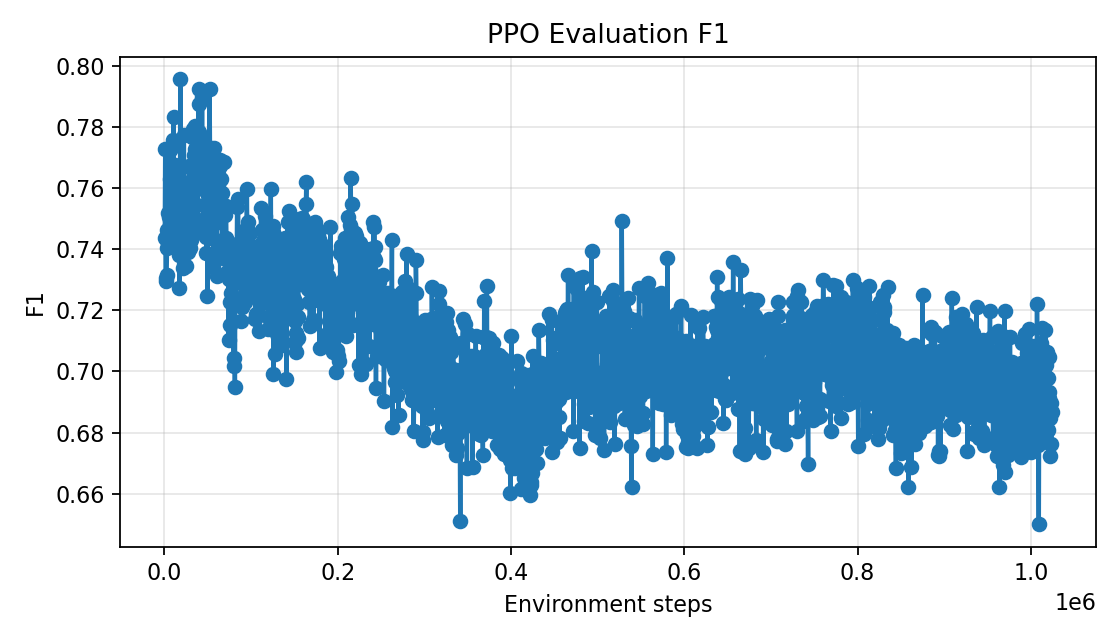
\includegraphics[width=0.78\linewidth]{docs/report_assets/ppo_petrunko_f1_curve.png}
\caption{Evaluation F1 curve for the \texttt{Petrunko\_3} single-song residual PPO baseline over 2000 iterations. The best checkpoint reaches F1 $=0.7957$ at 18,432 environment steps; the final saved rollout video is produced from this best checkpoint.}
\label{fig:ppo-f1-curve}
\end{figure}

\begin{table}[h]
\centering
\caption{Generalist diffusion checkpoint baseline on unseen test songs.}
\label{tab:generalist-baseline}
\begin{tabular}{lrrrr}
\toprule
Song & Split & Precision & Recall & F1 \\
\midrule
\texttt{Alone\_1} & test & 0.8283 & 0.6443 & 0.7902 \\
\texttt{Numb\_1} & test & 0.5286 & 0.4521 & 0.7504 \\
\texttt{NoTimeToDie\_1} & test & 0.8192 & 0.8076 & 0.8553 \\
\texttt{Forester\_1} & test & 0.8116 & 0.7300 & 0.7944 \\
\texttt{EyesClosed\_1} & test & 0.6127 & 0.5151 & 0.8569 \\
\texttt{Paradise\_1} & test & 0.8392 & 0.7535 & 0.8104 \\
\texttt{SomewhereOnlyWeKnow\_1} & test & 0.6516 & 0.5789 & 0.7920 \\
\bottomrule
\end{tabular}
\end{table}

\paragraph{Artifacts for qualitative comparison.}
All reproduced metrics, logs, videos, and the PPO curve are kept under
\texttt{/home/gaoj/share4/\_piano/baseline\_results}. The videos are currently
silent because the server lacks system-level FluidSynth/PortAudio libraries;
the visual simulation and note-level evaluation metrics are unaffected.
